\chapter{Conclusiones y recomendaciones}

Después de realizar este análisis la principal conclusión a la que se puede llegar es que si bien moodle es una base idónea para la gestión de la docencia online de la Universidad de Granada pensamos que se deberían realizar una serie de cambios y ajustes para adecuarlo a las necesidades propias de la Universidad.

\bigskip
Quiero hacer hincapié en el gran esfuerzo realizado por los profesionales del CEVUG y no quiero que este análisis se entienda como una crítica hacia su excelente trabajo. Con mi experiencia como desarrollador web puedo afirmar que no es fácil tener en cuenta los miles de detalles requeridos para personalizar, adaptar y optimizar una plataforma y mas cuando se trabaja a contrarreloj solucionando problemas lo que en muchos casos no permite mas que hacer un ajuste "temporal" que perdura en el tiempo indefinidamente. Por ello este informe, aunque dirigido a ellos como ayuda para optimizar la plataforma quizá debería servirles para hacer ver a sus superiores que algo tan importante como la plataforma web de apoyo a la docencia debería tener mas medios.

\bigskip
Sólo como nota, para gestionar su cuenta de twitter la policía nacional de España cuenta con un equipo de 8 personas a tiempo completo. Prado, que evidentemente es mas complejo y requiere muchísimo más trabajo solo cuenta con un desarrollador a tiempo completo y dos personas auxiliares a tiempo parcial.

\bigskip

La filosofía del software libre no se limita a distribuir software de forma gratuita, la idea es que al estar disponible el código fuente la gente pueda participar en el proyecto realizando modificaciones y mejoras. Si por el contrario nos limitamos a hacer uso del software sin aportar nada a la comunidad de desarrolladores estamos haciendo un flaco favor y además al venir esto de una institución donde se imparte conocimiento el efecto es aun mayor. Por lo pronto se debería mostrar de forma claro tanto que se está usando moodle como un enlace a su sitio original así como su licencia, cosa a la que de hecho obliga la licencia GPLv3 bajo la que está liberado moodle.

\bigskip

Es bien sabido en cualquier migración que los  indican en el libro de de MelenaAparte de eso partimos de la máxima de cada usuario es oponer resistencia al cambio y por lo tanto es obvio que iban a haber problemas con la migración a esta nueva plataforma.

Llevo muchos años trabajando en el mundo del desarrollo web y conozco sus dificultades por lo que me gustaría romper una lanza en favor de los administradores de Prado, pues  les ha tocado desempeñar una función con mucha dificultad y e


Los informáticos tenemos un deber con la sociedad, es complejo configurar la red eduroam


Es evidente que en el estado actual y con los recursos existentes no se puede competir con otras plataformas con muchos años a sus espaldas como puede ser SWAD, por eso quizá no sea mala idea en lugar de intentar acercarse a lo ya existente plantearse otro objetivo como puede ser la simplicidad. Como ya hemos visto la mayor parte de los usuarios necesitan un pequeño porcentaje de funciones. ¿Por qué no ocultar el resto? Imaginemos Prado como una plataforma basada en cuatro pilares fundamentales: Documentos, Tareas, Calificaciones y Mensajería. Si ocultamos el resto de opciones tenemos un sistema bastante más simple que el actual y seguramente sería suficiente para el 99\% de los usuarios.

Una vez realizada esta simplificación ya se podrían empezar a agregar funciones en base a su necesidad, pero sin olvidarnos de la máxima de la plataforma, que sería la simpleza. 


\section{Temporización final}

En la figura \ref{fig:temporizacion2} podemos ver un diagrama con los tiempos empleados para el desarrollo de este proyecto. 

\begin{figure}[H]
\centering
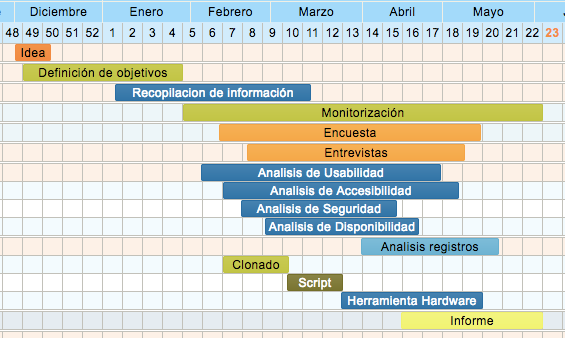
\includegraphics[width=0.8\textwidth]{../screenshots/temporizacion2}
\caption{Diagrama de Gantt con los tiempos invertidos en el proyecto}
\label{fig:temporizacion2}
\end{figure}

Los hitos más importantes en el desarrollo de este proyecto han sido los siguientes:

\begin{itemize}
	\item Septiembre 2014 - Primera contacto con Prado2

    \item Octubre 2016. Empieza a gestarse la idea de realizar un TFG sobre Prado2.
    
    \item Noviembre 2016. Se sientan las bases del proyecto. Se empiezan a recoger sugerencias de los usuarios.
    
    \item Enero 2016. Comenzamos a monitorizar la disponibilidad plataforma.
    
    \item Febrero 2016. Se lanza la encuesta a los usuarios de Prado.
    
    \item Marzo 2017 - Contactamos con los administradores de Prado2 para ver puntos de actuación en común y ver su punto de vista sobre la plataforma.
    
    \item Abril 2017. Se comienza a redactar la memoria.

    \item Mayo 2017. El CEVUG nos proporciona los logs de Prado.
    
    \item Junio 2017. Defensa final del proyecto

\end{itemize}




\newpage
En cuanto a futuras mejoras de la plataforma Prado2 vamos a clasificarlas las mejoras sugeridas en carácter urgente, recomendado y opcional:

\section{Mejoras de carácter urgente}

\begin{itemize}
	\item Configurar Prado para que sirva todo el contenido exclusivamente via HTTPS, para esto solo hay que activar la opción en la configuración de moodle y se conseguiría solucionar el problema de seguridad del secuestro de sesiones.


	\item Actualizar la versión de moodle, ya que en un entorno web en constante evolución no es admisible quedarse en versiones tan anticuadas ya que a la larga todo son problemas de compatiblidad. En el caso de Prado esto es aun mas


	
	


	\item Dejar todos los menús laterales visibles, ya que la implementación actual del template no respeta los anteriormente abiertos y crea mucha confusión al usuario al no saber donde se está
	
	\item Actualizar la versión de moodle 
	
	\item Bloquear en el fichero .htaccess el acceso a ficheros README y CHANGELOG,


\begin{lstlisting}
# ocultar archivos .txt, readmes, etc..
<IfModule mod_rewrite.c>
    RewriteCond %{REQUEST_URI} !/robots\.txt$ [nocase]
    RewriteRule \.txt$  -  [forbidden,last]
    RewriteRule \.xml$  -  [forbidden,last]
    RewriteRule \.md$  -  [forbidden,last]
</IfModule>
\end{lstlisting}	


	\item Activar los servicios web XML de moodle.
	
\end{itemize}


\section{Mejoras de carácter recomendado}

\begin{itemize}
	\item Forzar HTTPS en la configuración de moodle, y configurar el IDP para que retorne directamente a la pagina en https
	
\end{itemize}

\section{Mejoras de carácter opcional}
\begin{itemize}
	\item Forzar HTTPS en la configuración de moodle, y configurar el IDP para que retorne directamente a la pagina en https
	
\end{itemize}
